\subsection{DFR}
$x[k] = \frac{1}{N}$fft(x)

\subsection{DFT}
\subsubsection{X = fft(x)}
Bei Samplingfrequenz $f_s$ bekommt man für ein $T$-Langes Zeitsignal ein $f_s$-Langes Frequenzsignal mit Schritten $\frac{\Delta f}{T}$ \\
Achsensymmetrie bei $f=\frac{f_s}{2}$, achsensymmetr. für Realteil, punktsymmetr. für Imaginärteil \\
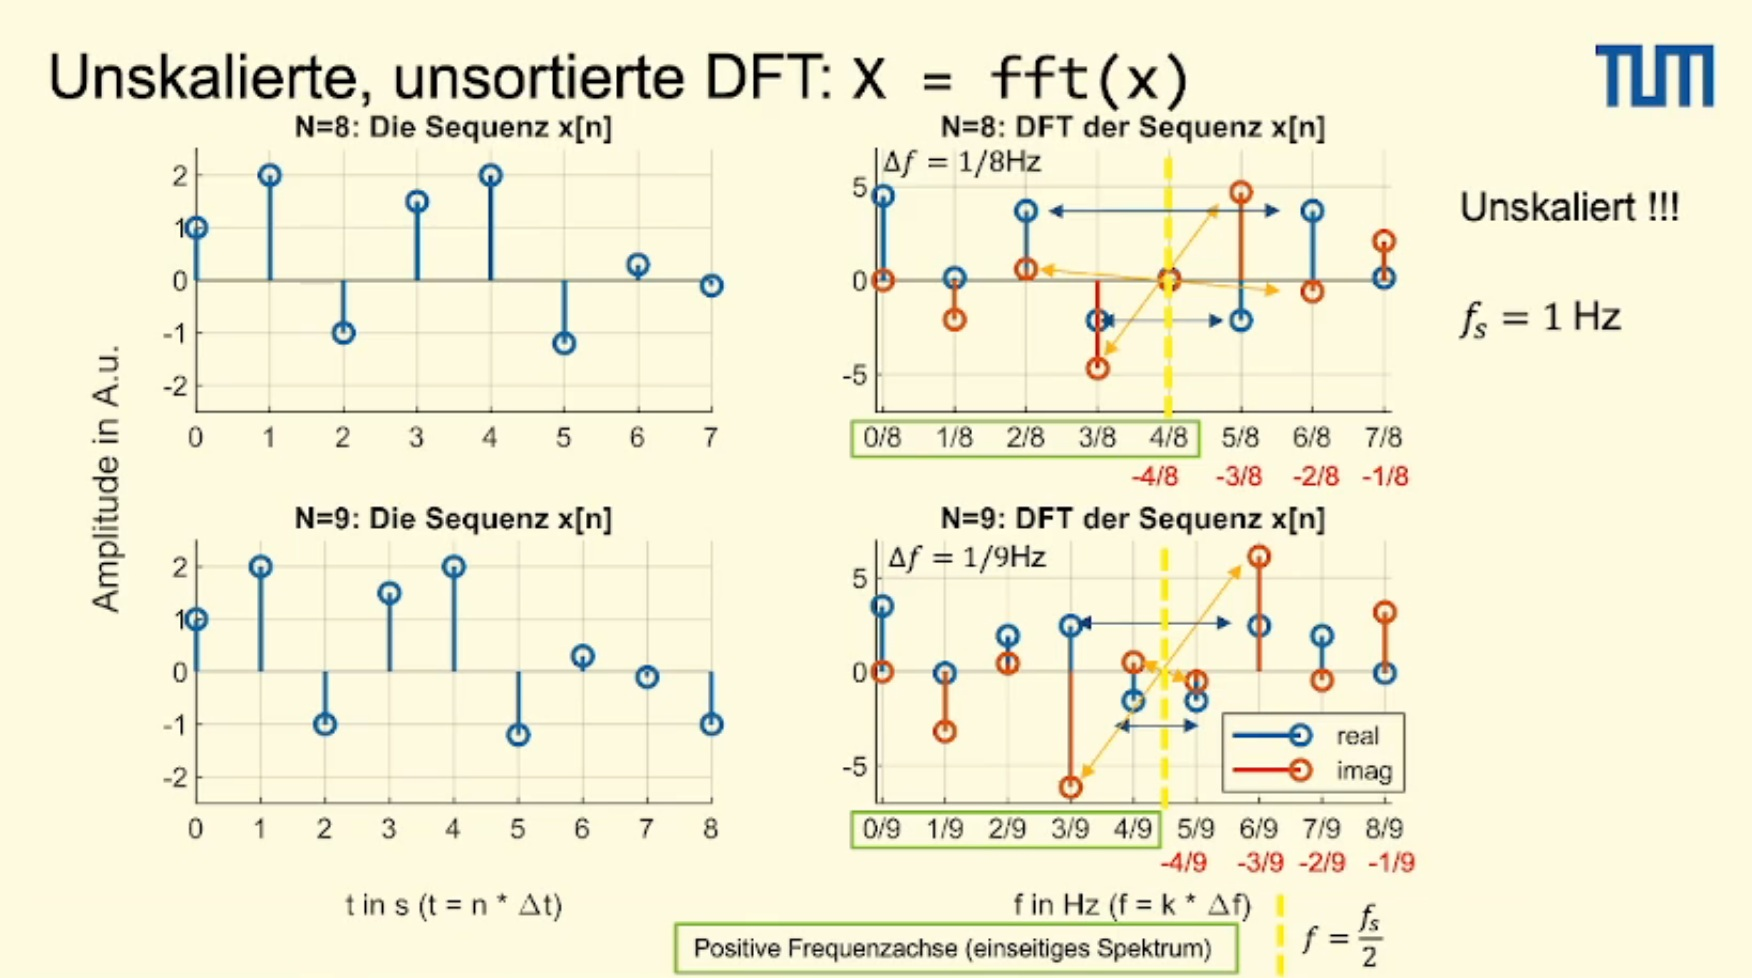
\includegraphics[width = \linewidth]{img/DFT-1.jpg}

\subsubsection{X = fftshift(fft(x))}
Signal wird so verschoben, dass es symmetr. um $f=0$ ist

TODO: Skalierung vom Amplitudenspektrum